\chapter{Analýza}
Tato kapitola pojednává o analýze aplikace. Výstupem této části jsou funkční, obecné požadavky, doménový model, aktéři a k nim případy užití.

\section{Požadavky}
Požadavky na systém se dělí na dvě sekce: obecné a funkční požadavky. Požadavky na systém jsem převzal z prototypu aplikace \citep{prototyp_documentace} a rozšířil jsem je o rozšířující specifikace zadavatele. Tyto požadavky mi definují návrh aplikace a technologie potřebné pro implementaci systému.

\subsection{Obecné požadavky}
Obecné požadavky se netýkají funkčnosti, ale celkového návrhu a použitých technologií.
\begin{enumerate}
\item Systém bude postaven na webovém frameworku Ruby on Rails.
\item Systém bude webovou aplikací.
\item Systém bude používat webovou službu KOSapi.
\item Systém bude pro autentizaci používat aplikaci FELid.
\end{enumerate}

\subsection{Funkční požadavky}
Tato sekce se zabývá požadavky na funkčnost systému.
\begin{enumerate}
\item Systém umožní průběžně plánovat hospitace.
\item Systém umožní hospitujícímu i hospitovanému prohlížet hospitace.
\item Systém umožní vystavit závěrečné hodnocení na veřejné části aplikace. 
\item Systém umožní hospitovanému sepsat stanoviska k názorům hospitujícího.
\item Systém umožní hospitujícímu nahrát naskenovaný dokument Hodnocení výuky.
\item Systém umožní hospitujícímu napsat slovní hodnocení z výuky.
\item Systém umožní hospitujícímu napsat závěrečné shrnutí hospitace.
\item Systém bude odesílat informačním emailem zprávy při vyplnění hodnotícího dokumentu.
\item Systém umožní vyhledávat předměty z KOSapi.
\item Systém umožní vyhledávat osoby z KOSapi.
\item Systém umožní upravovat strukturu hodnotících formulářů.
\item Systém umožní spravovat emailové šablony.
\item Systém umožní generovat emailové zprávy z emailových šablon.
\item Systém bude automaticky zálohovat databázi.
\end{enumerate}

\section{Uživatelské role}
V systému je celkem 7 uživatelských rolí. Definoval jsem čtyři základní uživatelské role, které jsou základem systému: nepřihlášený uživatel, přihlášený uživatel, administrátor hospitací a administrátor. Další dvě role hospitovaný a hospitující se přidělují v rámci konkrétních hospitací. Na obrázku \ref{fig:actors} jsou vidět jednotlivý aktéři a jejich zobecnění. V další části této sekce rozeberu jednotlivé role a k nim případy užití. Případy užití jsou obsaženy v příloze \ref{use_cases} tohoto dokumentu.

\paragraph*{Use cases}
neboli případy užití je nástroj pro popsání chování jak by systém měl spolupracovat s koncovým uživatelem. Popisuje všechny způsoby jak uživatel komunikuje se systémem.

\begin{figure}[H]
\begin{center}
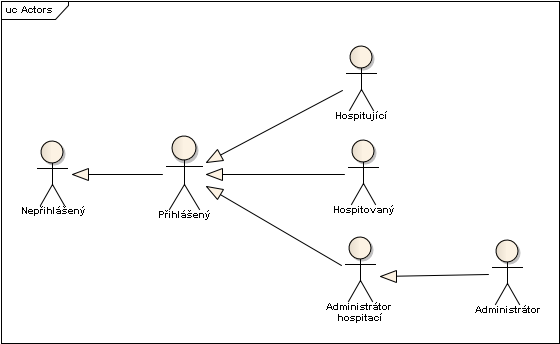
\includegraphics[width=10cm]{figures/Actors}
\caption{Aktéři}
\label{fig:actors}
\end{center}
\end{figure}

\subsection{Nepřihlášený uživatel}
Nepřihlášený uživatel je role pro hosty naší aplikace. V systému má ze všech rolí nejmenší pravomoc. V tomto stavu je každý uživatel, který se doposud nepřihlásil do systému. Případy užití pro nepřihlášeného uživatele jsou na obrázku \ref{fig:actor_base}.

\subsection{Přihlášený uživatel}
Přihlášený uživatel vychází z role nepřihlášeného uživatele. Je to uživatel, který se do systému přihlásil. Jedná se o základní roli pro všechny další role, které ji rozšiřují. Případy užití pro přihlášeného uživatele jsou na obrázku \ref{fig:actor_logged}.

\subsection{Hospitovaný}
Hospitovaný je role pro přihlášeného uživatele v systému. Je přidělena automaticky pro každého vyučujícího, který vyučuje předmět, na němž byla naplánovaná hospitace a tato hospitace proběhla. Případy užití pro hospitovaného jsou na obrázku \ref{fig:actor_observed}.

\subsection{Hospitující}
Hospitující je role pro přihlášeného uživatele v systému. Přiděluje se automaticky osobám, které mají za úkol vykonat hospitaci předmětu. Případy užití pro hospitujícího jsou na obrázku \ref{fig:actor_observer}.

\subsection{Administrátor hospitací}
Hlavním úkolem této role je plánovat hospitace na předměty a posléze je spravovat. Případy užití pro administrátora jsou na obrázku \ref{fig:actor_admin}.

\subsection{Administrátor}
Administrátor je super uživatel, který má nejvyšší pravomoc v systému. Má přístup ke všem zdrojům aplikace a může aplikaci spravovat. Případy užití pro administrátora jsou na obrázku \ref{fig:actor_root}.

\newpage 
\section{Doménový model}
Doménový model na obrázku \ref{fig:domainmodel} reprezentuje entity v systému a jejich vzájemné vztahy. Popis jednotlivých domény jsem pro přehlednost rozdělil podle zdroje na dvě základní skupiny. V první skupině jsou domény, které jsem převzal z RESTful rozhraní KOSapi\footnote{viz. \ref{kosapi}} a druhou skupinou jsou domény specifické pro moji aplikaci. 

\label{sec:domeny_kosapi} 
\subsection{Domény v KOSapi}
\begin{itemize}
\item Osoba - je osoba v KOSu. Každá osoba může být učitelem a studentem.
\item Semestr - semestr vyučovaný na FEL. 
\item Předmět - předměty vyučované na FEL.
\item Instance předmětu - jsou instance předmětu vypsané v konkrétním semestru.
\item Paralelka - je vypsaná rozvrhová paralelka pro instanci předmětu.
\item Místnost - místnost na FEL
\end{itemize}

\subsection{Domény aplikace}
\begin{itemize}
\item Hospitace - obsahuje informace o naplánování hospitace. 
\item Poznámka - je textová poznámka k plánování hospitace.
\item Hodnocení - reprezentuje informace z proběhlé hospitace hospitace, jsou to informace o datu vykonání hospitace, hospitujícím, předmětu a garantovi.
\item Příloha - je připojený datový soubor k hodnocení hospitace.
\item Šablona formuláře - šablona pro tvorbu formulářů. Definuje vlastnosti jakým se budou vytvářet hodnotící formuláře.
\item Položka - položka reprezentuje jednotlivé segmenty formuláře. Tyto segmenty pak v celku definují strukturu formuláře.
\item Formulář - vyplněný hodnotící formulář.
\item Hodnota - je hodnota z vyplněného formuláře. Ta se ukládá z položky formuláře.
\item Šablona emailu - šablona emailu ze které se budou generovat emailové zprávy.
\end{itemize}

\begin{figure}[p]
\begin{center}
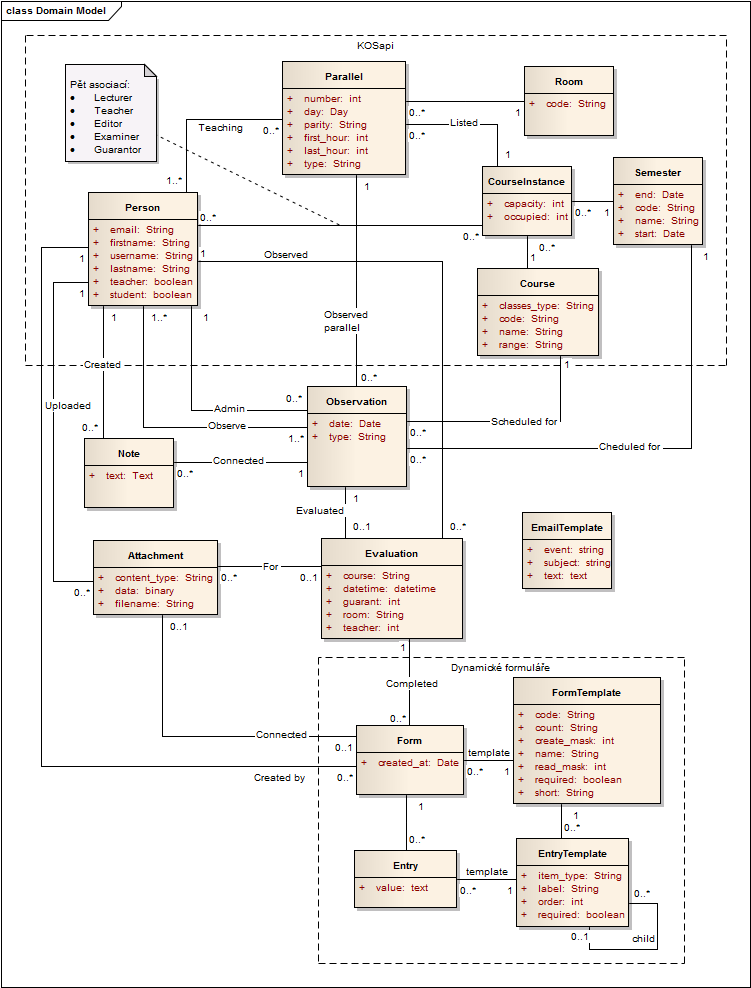
\includegraphics[width=14cm]{figures/DomainModel2}
\caption{Doménový model}
\label{fig:domainmodel}
\end{center}
\end{figure}


\newpage 
\section{Průběh hospitace}
Cílem této části analýzy je popsat průběh hospitace od jejího vytvoření po ukončení. Průběh hospitace je graficky zobrazený na diagramu \ref{fig:hospitace}.

\subsection{Vytvoření}
Životní cyklus hospitace začíná jejím vytvořením. V této fázi účinkuje pouze aktér administrátor hospitací. Při vytváření hospitace je potřeba definovat: předmět, semestr a typ hospitace\footnote{definuje způsob zviditelnění, pro ostatní aktéry v aplikaci}. Po úspěšném vytvoření hospitace následuje fáze plánování.

\subsection{Plánování}
Při plánování je také hlavním aktérem administrátor hospitace. V této části životního cyklu administrátor určí paralelku předmětu a datum uskutečnění hospitace. V této fázi musí administrátor hospitací přidělit hospitujícího.  
 
\subsection{Hodnocení}
Po vykonání kontrolní návštěvy začíná nová fáze hodnocení vyučování. V této fázi již neúčinkuje administrátor hospitace, ale přicházejí na scénu aktéři hospitovaný a hospitující. Hodnocení probíhá postupným vyplňováním hodnotících formulářů. 
\begin{enumerate}
\item Hospitující musí vyplnit, nebo nahrát naskenovaný formulář Hodnocení výuky při hospitaci. Tento formulář slouží k dokumentaci průběhu hospitace.
\item Jeden z hospitujících sepíše Slovní hodnocení hospitační návštěvy.
\item Pokud hospitovaný se chce vyjádřit k hospitaci, může vyplnit formulář Stanovisko hodnoceného k názorům hospitujícího.
\item Jeden z hospitujících sepíše formulář Závěrečné shrnutí.
\end{enumerate}
 
\subsection{Ukončená}
Po vyplnění posledního formuláře Závěrečné shrnutí je hospitace ve stavu ukončená a tím končí i její životní cyklus.

\begin{figure}[h]
\begin{center}
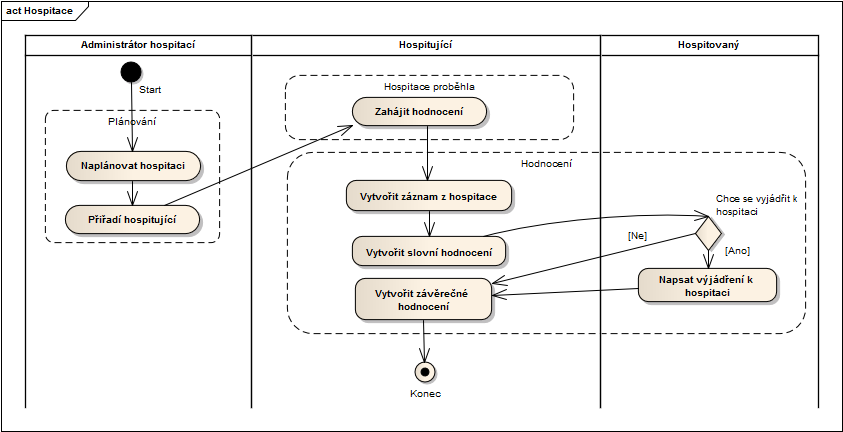
\includegraphics[height=10cm,angle=270]{figures/hospitace}
\caption{Průběh hospitace}
\label{fig:hospitace}
\end{center}
\end{figure}
